% Frugal AI seminar, project 3: fine-tuning a small model on a CPU (FrugalAI/code/finetune-slm).
% Procedure and theory only, no results. CheatSheet-safe: no floats.

\section[CPU Fine-Tune]{Project: Fine-Tuning on a CPU}

%%%%%%%%%%%%%%%%%%%%%%%%%%%%%%%%%%%%%%%%%%%%%%%%%%%
\begin{frame}[fragile]\frametitle{}
\begin{center}
{\Large Project: Fine-Tuning a Small Model on a CPU}

\medskip
{\small (Teach a small open model a book or a narrow job, without a GPU)}
\end{center}
\end{frame}

%%%%%%%%%%%%%%%%%%%%%%%%%%%%%%%%%%%%%%%%%%%%%%%%%%%
\begin{frame}[fragile]\frametitle{Theory: LoRA and Why It Fits a CPU}
\begin{itemize}
\item Full fine-tuning updates every weight and needs memory for gradients and optimiser state of the whole model. That rules out most laptops.
\item LoRA (low-rank adaptation) freezes the base weights and trains small added matrices next to chosen layers. Only those matrices get gradients.
\item The trainable share is typically a few percent of the model or less, so memory and time drop sharply. The result is a small adapter file, not a new model.
\item Settings that matter: the rank and alpha of the added matrices, which layers get them (attention only, or also the feed-forward layers), the learning rate, the number of epochs.
\item Fine-tuning moves cost from every request to one training run. It pays off when the task is stable and repeated.
\end{itemize}
{\tiny (Ref: Hu et al., LoRA; Hugging Face PEFT)}
\end{frame}

%%%%%%%%%%%%%%%%%%%%%%%%%%%%%%%%%%%%%%%%%%%%%%%%%%%
\begin{frame}[fragile]\frametitle{Procedure: Check, Build, Train, Test}
\begin{center}
\adjustbox{max width=0.97\linewidth, max totalheight=0.2\textheight}{%
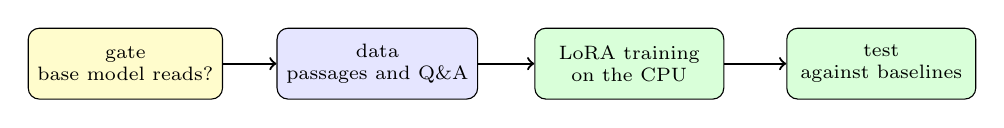
\begin{tikzpicture}
\tikzstyle{b}=[draw, rounded corners, align=center, minimum height=0.9cm, minimum width=2.4cm, font=\scriptsize]
\node[b, fill=yellow!20] (g) at (0,0) {gate\\base model reads?};
\node[b, fill=blue!10] (d) at (3.2,0) {data\\passages and Q\&A};
\node[b, fill=green!15] (t) at (6.4,0) {LoRA training\\on the CPU};
\node[b, fill=green!15] (e) at (9.6,0) {test\\against baselines};
\draw[->, thick] (g) -- (d);
\draw[->, thick] (d) -- (t);
\draw[->, thick] (t) -- (e);
\end{tikzpicture}}
\end{center}
\begin{itemize}
\item Gate first. Before any training, test the base model: can it answer from a passage placed in the prompt, in the target language? If it cannot read, training on a small text will not fix that.
\item Measure how many tokens a word costs in the model's tokenizer. A high number means long sequences and slow training.
\item Compare the tuned model with two honest alternatives on the same questions: the base model alone, and the base model reading retrieved passages.
\end{itemize}
{\tiny (Ref: FrugalAI code/finetune-slm)}
\end{frame}

%%%%%%%%%%%%%%%%%%%%%%%%%%%%%%%%%%%%%%%%%%%%%%%%%%%
\begin{frame}[fragile]\frametitle{Implementation: Data and a Fair Test}
\begin{itemize}
\item Two kinds of training example in one run. Raw passages, with the loss on every token, teach the text. Question and answer pairs in the chat format, with the loss on the answer only, teach the answering style.
\item Passages are cut at paragraph boundaries, about 90 words each, and headed with the chapter title so facts attach to their chapter.
\item A closed-book model cannot be tested on text it never saw. So hold out the wording, not the text: ask old facts in new words, ask about facts that appear only in the raw text, and add a control group about chapters withheld from training.
\item Check mechanically that every answer key occurs in its chapter, that no test question appears in the training data, and that withheld chapters have no training item.
\item Score with key phrases that must appear in the answer, and read a sample by eye. Fluent text is not correct text.
\end{itemize}
{\tiny (Ref: FrugalAI code/finetune-slm, mrsj)}
\end{frame}

%%%%%%%%%%%%%%%%%%%%%%%%%%%%%%%%%%%%%%%%%%%%%%%%%%%
\begin{frame}[fragile]\frametitle{Implementation: Training on a Laptop CPU}
\begin{itemize}
\item Plain PyTorch loop with the PEFT library: load the model, wrap it with a LoRA config, train, save the adapter. Hide the GPU so the run reflects a CPU-only machine.
\item Use float32 on a CPU. Half-precision formats can be extremely slow on processors without native support.
\item Set the thread count to the physical cores. Use batch size one with gradient accumulation to keep memory low; a large vocabulary makes the output layer the biggest memory item.
\item Check free memory before starting and refuse to run if it is too low. A job that exhausts memory is stopped by the system and loses its work.
\item Save progress every few dozen examples (adapter plus a small state file) and resume mid-epoch. Keep each finished epoch as its own folder so any epoch can be evaluated.
\item Serve the result by merging the adapter, converting to GGUF, and calling it from LangChain like any other local chat model.
\end{itemize}
{\tiny (Ref: Hugging Face PEFT and Transformers; FrugalAI code/finetune-slm)}
\end{frame}
